%==============================================================================
%  SurroForge — Pitch-Präsentation
%  Spezifikation: PRD.md  |  LaTeX Beamer, 16:9, Deutsch, 8 Folien
%  Kompilieren:  latexmk -pdf surroforge.tex      (oder 2x pdflatex surroforge.tex)
%
%  Ohne Sprechernotizen (laut PRD: Pitch-Termin, 8 Min Vortrag).
%==============================================================================
\documentclass[aspectratio=169,11pt]{beamer}

%--- Schrift (laut PRD: Sans fuer Body, Serif fuer Titel, Mono fuer Code) -------
\usepackage[T1]{fontenc}
\usepackage[utf8]{inputenc}
\usepackage[ngerman]{babel}
\usepackage{sourceserifpro}          % Serif (Titel)         -> \rmfamily
\usepackage[sfdefault]{FiraSans}     % Sans  (Body, Default)
\usepackage[scaled=0.84]{FiraMono}   % Mono  (Code)          -> \ttfamily
\usepackage{textcomp}
\usepackage{pifont}
\usepackage{fontawesome5}             % Branchen-Icons (Folie 6)
\usepackage{microtype}

\usefonttheme{professionalfonts}     % Beamer ersetzt unsere Schriften nicht
\setbeamertemplate{navigation symbols}{}

%--- Grafik ---------------------------------------------------------------------
\usepackage{tikz}
\usetikzlibrary{positioning,arrows.meta,calc,backgrounds,fit}
\usepackage[most]{tcolorbox}

%==============================================================================
%  Farbpalette  —  zurueckhaltend, technisch-professionell
%  Primaer: Anthrazit-Navy | Akzent: Terracotta + Bernstein (sparsam)
%==============================================================================
\definecolor{sfnavy}{HTML}{1E2A36}   % Primaer dunkel (Anthrazit-Navy)
\definecolor{sfink}{HTML}{232B33}     % Fliesstext
\definecolor{sfslate}{HTML}{596570}   % Sekundaertext / Linien
\definecolor{sfmute}{HTML}{8A929A}    % gedaempft
\definecolor{sfaccent}{HTML}{BF6438}  % Terracotta (Haupt-Akzent)
\definecolor{sfamber}{HTML}{D49A3A}   % Bernstein (sehr sparsam)
\definecolor{sfpaper}{HTML}{F6F3EE}   % warmes Off-White (Hintergrund)
\definecolor{sfrule}{HTML}{E2DBCF}    % warme helle Linie
\definecolor{sfcard}{HTML}{FFFFFF}

%--- Beamer-Farben --------------------------------------------------------------
\setbeamercolor{normal text}{fg=sfink,bg=sfpaper}
\setbeamercolor{structure}{fg=sfaccent}
\setbeamercolor{frametitle}{fg=sfnavy,bg=}
\setbeamercolor{itemize item}{fg=sfaccent}
\setbeamercolor{itemize subitem}{fg=sfmute}
\setbeamercolor{alerted text}{fg=sfaccent}
\setbeamerfont{frametitle}{series=\bfseries}

%--- Aufzaehlungs-Marker (kleines Akzent-Quadrat) -------------------------------
\setbeamertemplate{itemize item}{\raisebox{0.28ex}{\color{sfaccent}\rule{0.55ex}{0.55ex}}}
\setbeamertemplate{itemize subitem}{\raisebox{0.18ex}{\color{sfmute}\rule{0.42ex}{0.42ex}}}
\setbeamertemplate{itemize/enumerate body begin}{\small}
\setbeamertemplate{enumerate items}[default]
\setbeamercolor{enumerate item}{fg=sfaccent}

%==============================================================================
%  Frametitel:  Serif, Navy, duenne Akzent-Linie darunter
%==============================================================================
\setbeamertemplate{frametitle}{%
  \nointerlineskip\vskip0.5em%
  {\rmfamily\bfseries\color{sfnavy}\large\strut\insertframetitle\par}%
  \vskip3pt{\color{sfaccent}\rule{1.5em}{2.2pt}}\par\vskip2pt%
}

%==============================================================================
%  Footer:  Mini-Surrogate-Motiv + Wortmarke + Seitenzahl
%==============================================================================
\newcommand{\footmotif}{%
  \begin{tikzpicture}[baseline=-0.4ex]
    \draw[sfaccent,line width=0.8pt] (0,0) .. controls (0.28,0.34) and (0.62,-0.06) .. (0.95,0.2);
    \foreach \p in {(0,0),(0.32,0.22),(0.63,0.02),(0.95,0.2)}{\fill[sfnavy] \p circle (1.3pt);}
  \end{tikzpicture}}
\setbeamertemplate{footline}{%
  \hbox{\begin{beamercolorbox}[wd=\paperwidth,ht=2.6ex,dp=1.5ex,leftskip=1.4em,rightskip=1.4em]{}%
    \footmotif\hspace{0.7em}{\footnotesize\color{sfslate}\textbf{SurroForge}}%
    \hfill{\footnotesize\color{sfmute}Projektpitch · Validierungsphase}%
    \hfill{\footnotesize\color{sfslate}\insertframenumber}%
  \end{beamercolorbox}}%
}

%==============================================================================
%  Hilfsmakros
%==============================================================================
\newcommand{\rarr}{\textcolor{sfslate}{\,\textrightarrow\,}}
\newcommand{\cmark}{\textcolor{sfaccent}{\ding{51}}}
\newcommand{\gq}[1]{\glqq #1\grqq{}}
\newcommand{\Rsq}{R\textsuperscript{2}}
\newcommand{\lead}[1]{{\rmfamily\color{sfnavy}#1}}

%--- Karten (tcolorbox) mit Titelband ------------------------------------------
\newtcolorbox{cardbox}[2][sfnavy]{%
  enhanced,colback=sfcard,colframe=sfrule,boxrule=0.8pt,arc=2pt,halign=left,
  coltitle=sfcard,colbacktitle=#1,fonttitle=\rmfamily\bfseries\small,
  title={#2},left=8pt,right=8pt,top=5pt,bottom=7pt,
  before skip=2pt,after skip=2pt}

%--- Terminal-/CLI-Box ----------------------------------------------------------
\definecolor{termbg}{HTML}{222E3A}
\definecolor{termfg}{HTML}{E8E2D6}
\newtcolorbox{terminal}{enhanced,colback=termbg,colframe=termbg,boxrule=0pt,
  arc=3pt,left=12pt,right=12pt,top=10pt,bottom=10pt,
  before skip=4pt,after skip=4pt}

%--- TikZ-Stile -----------------------------------------------------------------
\tikzset{
  chip/.style={rounded corners=2pt,draw=sfrule,line width=0.8pt,fill=sfcard,
               font=\scriptsize,text=sfink,inner sep=4pt,align=center},
  flow/.style={-{Stealth[length=2mm]},sfslate,line width=1pt},
  dashflow/.style={-{Stealth[length=2mm]},sfmute,line width=0.9pt,dashed},
  node distance=5mm and 7mm,
}

%--- Metadaten ------------------------------------------------------------------
\title{SurroForge}
\subtitle{Effiziente ML-Surrogate-Modelle für FEM und CFD}
\author{Georg Babij}                 % TODO: Name/Kontakt anpassen
\date{Mai 2026}

%==============================================================================
%  DOKUMENT
%==============================================================================
\begin{document}

%------------------------------------------------------------------ Folie 1 ----
{%
\setbeamercolor{background canvas}{bg=sfnavy}
\begin{frame}[plain]
  % Hintergrund-Motiv: Stichproben + glatte Surrogate-Kurve
  \begin{tikzpicture}[remember picture,overlay]
    \begin{scope}[shift={($(current page.north east)+(-4.9,-3.2)$)},scale=0.82]
      \draw[sfslate!55,line width=0.6pt] (0,0) -- (4.6,0);
      \draw[sfslate!55,line width=0.6pt] (0,0) -- (0,2.6);
      \draw[sfaccent,line width=1.6pt]
        (0,0.5) .. controls (1.0,2.0) and (1.8,0.6) ..
        (2.6,1.6) .. controls (3.3,2.4) and (4.0,1.9) .. (4.6,2.3);
      \foreach \p in {(0,0.5),(0.9,1.55),(1.7,0.75),(2.6,1.6),(3.4,2.1),(4.2,2.15)}
        {\fill[sfpaper] \p circle (3pt); \draw[sfnavy,line width=0.8pt] \p circle (3pt);}
    \end{scope}
  \end{tikzpicture}

  \vspace{1.6cm}
  \hspace{0.4cm}\color{sfamber}\rule{2.2em}{3pt}\par
  \vspace{0.5em}
  {\hspace{0.4cm}\rmfamily\bfseries\color{sfpaper}\fontsize{46}{50}\selectfont SurroForge\par}
  \vspace{0.8em}
  {\hspace{0.42cm}\color{sfpaper}\large ML-Surrogate-Modelle in der MDAO-Optimierung\par}
  \vspace{1.8cm}
  {\hspace{0.42cm}\color{sfmute}\small Erstellung aus FEM, CFD und experimentellen Daten \ \textbar\ Open-Core \ \textbar\  CLI-Tool}\par
  \vspace{0.3em}
  {\hspace{0.42cm}\color{sfmute}\footnotesize Projektpitch · Validierungsphase · Mai 2026}\par
\end{frame}
}

%------------------------------------------------------------------ Folie 2 ----
\begin{frame}[t]{Der Schmerz in der Optimierung (MDAO) — und warum jetzt}
  \begin{columns}[t]
    \begin{column}{0.56\textwidth}
      \begin{itemize}\setlength\itemsep{0.4em}
        \item Performanz der Simulationsmodelle \alert{schwach}:  Zeitverlust in \alert{MDAO-Workflows} durch
              bei FEM, CFD (HiFi) \& Ungenauigkeit bei bisherigen Surrogate-Modellen (LoFi).
        \item Tools und Datenquellen jedes Mal neu zu verbinden
              \alert{kostet Zeit und erzeugt Fehler}.
        \item Methodenwissen steckt in \alert{einzelnen Köpfen}.
      \end{itemize}
      \vspace{0.25em}
      \begin{cardbox}[sfaccent]{Warum jetzt}
        \footnotesize
        AI-Hype trifft im Engineering auf ein reifes Methoden-Ökosystem
        (SMT, GPyTorch) — \textbf{das Standardwerkzeug darüber fehlt}.
      \end{cardbox}
    \end{column}
    \begin{column}{0.44\textwidth}
      \centering\vspace{0.2em}
      \begin{tikzpicture}[baseline=(current bounding box.north)]
        \node[inner sep=0pt,draw=sfrule,line width=0.8pt]
              {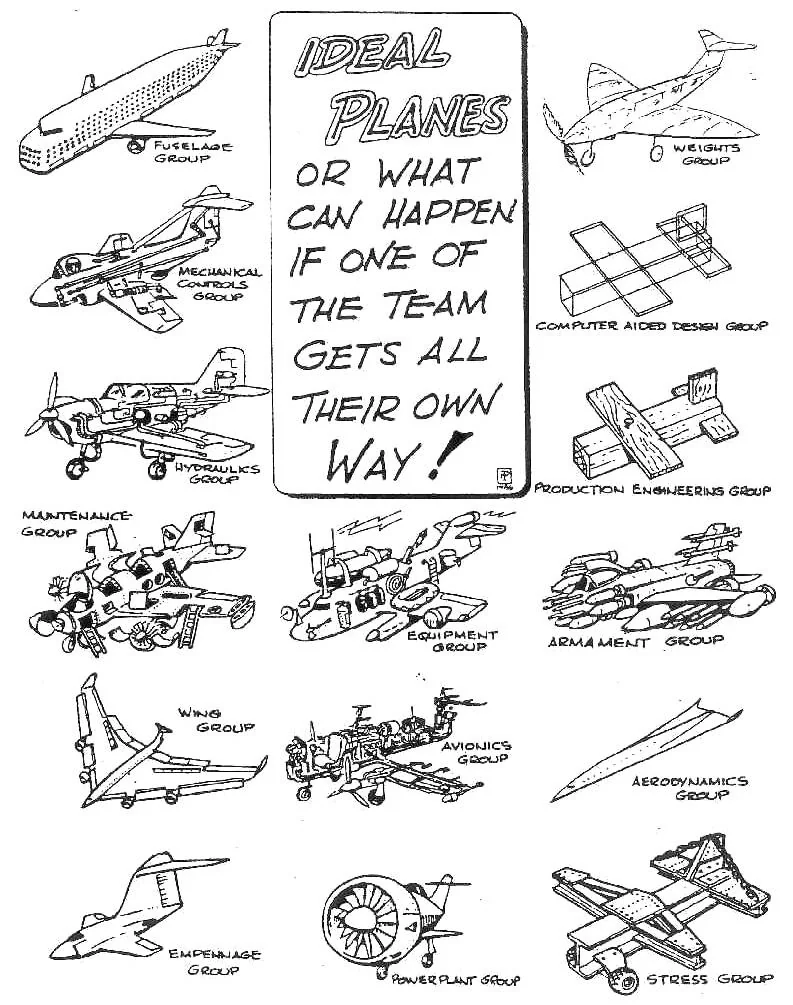
\includegraphics[height=5.2cm]{the-ideal-plane.png}};
      \end{tikzpicture}\\[3pt]
      {\scriptsize\color{sfaccent}Jede Disziplin ihr eigenes Optimum — niemand das Gesamtsystem.}
    \end{column}
  \end{columns}
\end{frame}

%------------------------------------------------------------------ Folie 3 ----
\begin{frame}[t]{Die Lösung — ein fokussiertes CLI}
  \begin{columns}[t]
    \begin{column}{0.46\textwidth}
      {\small Von Input-Daten (FEM/CFD/Experiment) zum validierten
      ML-Surrogate in unter einer Stunde.}\\[10pt]
      {\small SurroForge bündelt \textbf{Standardisierung}, \textbf{Reproduzierbarkeit}
      und \textbf{Methoden-Vergleich} in einem schlanken CLI.}\\[10pt]
      {\small\textbf{Fokus:} schnelle \& reproduzierbare Surrogate, die sich in
      \textbf{bestehende Workflows} integrieren.}
    \end{column}
    \begin{column}{0.54\textwidth}
      \begin{terminal}
        \ttfamily\scriptsize\color{termfg}
        \textcolor{sfamber}{\$}\ surroforge fit doe.csv {-}{-}target spannung \textbackslash\\
        \hspace{1.4em}{-}{-}methods kriging,rbf,gp {-}{-}cv 5\\[6pt]
        \color{sfmute}\# trainiert, kreuzvalidiert, vergleicht\\[6pt]
        \cmark\ 3 Modelle · bestes: \textcolor{termfg}{kriging} (\Rsq\ = 0.982)\\
        \cmark\ Report\ \rarr\ report.html\\
        \cmark\ Modell\ \rarr\ model.sfm \textcolor{sfmute}{(versioniert)}
      \end{terminal}
      \vspace{2pt}
      {\scriptsize\color{sfslate}Ein Aufruf: mehrere Methoden, ehrliche Cross-Validation,
      ein versioniertes Artefakt, das morgen dasselbe Ergebnis liefert.}
    \end{column}
  \end{columns}
\end{frame}

%------------------------------------------------------------------ Folie 4 ----
\begin{frame}[t]{Zielnutzer und Käufer — gleiche Krankheit}
  \begin{columns}[t]
    \begin{column}{0.5\textwidth}
      \begin{cardbox}[sfnavy]{Nutzer · Methodeningenieur}
        \footnotesize
        \textit{\gq{Ich will Modelle bauen, nicht Skripte debuggen.}}\\[3pt]
        \textbf{Zentraler Schmerz:} Zeitverlust durch ineffiziente
        Surrogate-Modelle und fragmentierte Tools.\\[3pt]
        \textbf{Gewinn:} schneller zum validierten ML-Surrogate — reproduzierbar und teilbar.
      \end{cardbox}
    \end{column}
    \begin{column}{0.5\textwidth}
      \begin{cardbox}[sfaccent]{Käufer · Leitung MDAO-Abteilung}
        \footnotesize
        \textit{\gq{Wissen darf nicht an einzelnen Köpfen hängen.}}\\[3pt]
        \textbf{Strategischer Hebel:} Wissenssicherung und Effizienzsteigerung —
        Standardisierung statt Schlüsselpersonen-Risiko.\\[3pt]
        \textbf{Gewinn:} verlässliche, vergleichbare Auslegung als Team-Standard.
      \end{cardbox}
    \end{column}
  \end{columns}
  \vspace{0.3em}
  \begin{center}
    \begin{tikzpicture}
      \node[font=\footnotesize,text=sfslate] (l) {Nutzer: \textbf{verlorene Zeit}};
      \node[draw=sfaccent,rounded corners=2pt,fill=sfaccent!10,font=\footnotesize\bfseries,
            text=sfnavy,inner sep=5pt,right=8mm of l] (m) {gleiche Krankheit};
      \node[font=\footnotesize,text=sfslate,right=8mm of m] (r) {Käufer: \textbf{Risiko \& Wildwuchs}};
      \draw[flow] (l) -- (m); \draw[flow] (m) -- (r);
    \end{tikzpicture}\\[1pt]
    {\scriptsize\color{sfmute}Ein Problem, zwei Symptome — zwei Argumente im selben Haus.}
  \end{center}
\end{frame}

%------------------------------------------------------------------ Folie 5 ----
\begin{frame}[t]{Geschäftsmodell — Open Core als bewusste Wahl}
  \begin{columns}[t]
    \begin{column}{0.33\textwidth}
      \begin{cardbox}[sfslate]{Core · Open Source}
        \scriptsize
        Fit · Validate · Compare in der \textbf{CLI}. Kein GUI/Optimierer.\\[4pt]
        \textbf{Frei} \rarr\ Adoption.
      \end{cardbox}
    \end{column}
    \begin{column}{0.33\textwidth}
      \begin{cardbox}[sfaccent]{Professional}
        \scriptsize
        Team-Reporting, Integrationen, \textbf{GUI-Add-on}, Support.\\[4pt]
        \textbf{Abo / Seat} \rarr\ erster Umsatz.
      \end{cardbox}
    \end{column}
    \begin{column}{0.33\textwidth}
      \begin{cardbox}[sfnavy]{Enterprise}
        \scriptsize
        Governance, On-Prem, SSO, SLA, \textbf{Optimierungssolver}.\\[4pt]
        \textbf{Vertrag} \rarr\ Skalierung.
      \end{cardbox}
    \end{column}
  \end{columns}
  \vspace{0.3em}
  \centerline{\begin{tikzpicture}[font=\scriptsize,every node/.style={align=center}]
      \node[text=sfslate] (a) {Einzelner\\probiert Core};
      \node[text=sfslate,right=10mm of a] (b) {Team braucht\\Reporting \& Support};
      \node[text=sfslate,right=10mm of b] (c) {Organisation fordert\\Governance \& SLA};
      \draw[flow] (a) -- (b); \draw[flow] (b) -- (c);
  \end{tikzpicture}}
  \vspace{0.3em}
  \begin{cardbox}[sfaccent]{Strategischer Vorteil}
    \small \textbf{Offener Kern, geschlossenes Herz:} freier CLI-Kern; \textbf{GUI
    \& Optimierungssolver} als zukaufbare Add-ons — so entstehen \textbf{Vertrauen}
    und \textbf{Monetarisierung}.
  \end{cardbox}
\end{frame}



%------------------------------------------------------------------ Folie 6 ----
{%
\setbeamercolor{background canvas}{bg=sfnavy}
\setbeamercolor{normal text}{fg=sfpaper,bg=sfnavy}
\usebeamercolor[fg]{normal text}
\begin{frame}[t]
  \vspace{0.3em}
  {\hspace{0.3cm}\rmfamily\bfseries\color{sfpaper}\large Drei Gründe, warum SurroForge relevant ist}\\[2pt]
  {\hspace{0.32cm}\color{sfaccent}\rule{1.5em}{2.2pt}}
  \vspace{0.4em}

  \hspace{0.3cm}\begin{minipage}{0.93\textwidth}
  \color{sfpaper}\small
  \begin{enumerate}\setlength\itemsep{0.3em}
    \item In \textbf{Optimierungsabteilungen (MDAO)} gibt es einen \textbf{teuren
          Schmerz}: kostspielige High-fidelity-Simulationen, ineffiziente
          Surrogate-Modelle, Wissensengpässe.
    \item \textbf{SurroForge adressiert ihn fokussiert} — ein CLI für
          Standardisierung, Reproduzierbarkeit und Methoden-Vergleich.
    \item \textbf{Open Core, bewusst gewählt} — offener Kern, geschlossenes Herz:
          Adoption über den freien Kern, Erlös über Professional und Enterprise.
  \end{enumerate}
  \end{minipage}

  \vfill
  {\hspace{0.32cm}\color{sfmute}\footnotesize Kontakt: Georg Babij · g.babij@googlemail.com\ \textbar\ Nächster Schritt: Validierungs-Interviews}
  \vspace{0.4em}
\end{frame}
}

\end{document}
